\documentclass{standalone}
\usepackage{mathpazo}
\usepackage{siunitx}
\usepackage[american voltages, american currents, american inductors]{circuitikz}
\newcommand*{\equal}{=}

\begin{document}
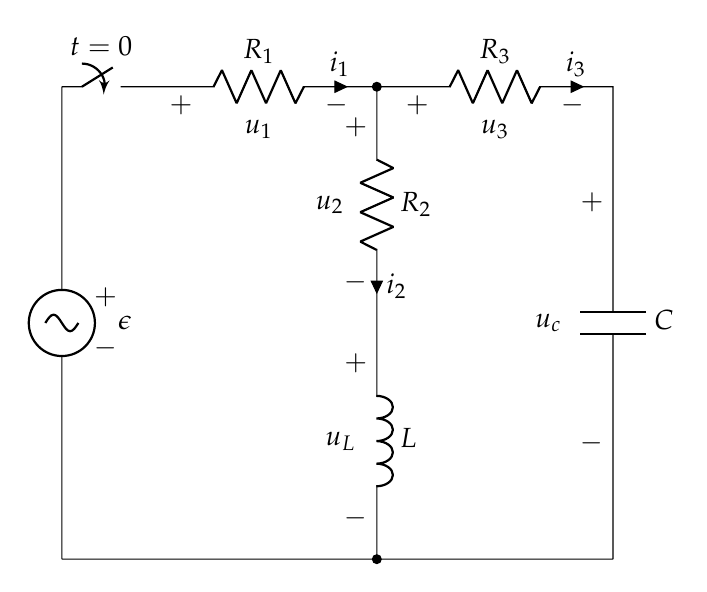
\begin{tikzpicture}
  \coordinate (A) at (0,6);
  \coordinate (B) at (4,6);
  \coordinate (C) at (7,6);
  \coordinate (D) at (0,0);
  \coordinate (E) at (4,0);
  \coordinate (F) at (7,0);
  \draw
  (A) to [closing switch, l = $t \equal 0$] ++(1,0)
  to [R, l = $R_1$, v = $u_1$, i = $i_1$, -*] (B)
  (D) to [short, -*] (E)
  to [short, -] (F)
  (A) to [sV, v = $\epsilon$] (D)
  (B) to [R, l = $R_2$, v = $u_2$, i = $i_2$] ++(0, -3)
  to [L, l = $L$, v = $u_L$] (E)
  (B) to [R, l = $R_3$, i= $i_3$, v = $u_3$] (C)
  to [C, l = $C$, v = $u_c$] (F);
  \end{tikzpicture}
\end{document}